\documentclass[a0paper,portrait]{baposter}
\usepackage{wrapfig}
\usepackage{lmodern}
\usepackage[utf8]{inputenc} %unicode support
\usepackage[T1]{fontenc}
\selectcolormodel{cmyk}
\graphicspath{{figures/}} % Directory in which figures are stored
\newcommand{\compresslist}{%
\setlength{\itemsep}{0pt}%
\setlength{\parskip}{1pt}%
\setlength{\parsep}{0pt}%
}
\newenvironment{boenumerate}
  {\begin{enumerate}\renewcommand\labelenumi{\textbf\theenumi.}}
  {\end{enumerate}}
\begin{document}
\definecolor{alizarin}{rgb}{0.82, 0.1, 0.26}
\definecolor{airforceblue}{rgb}{0.36, 0.54, 0.66}
\definecolor{babypink}{rgb}{0.96, 0.76, 0.76}
\definecolor{darkgreen}{cmyk}{0.8,0,0.8,0.45}
\definecolor{lightgreen}{cmyk}{0.8,0,0.8,0.25}
\definecolor{aqua}{rgb}{0.0, 1.0, 1.0}
\definecolor{amethyst}{rgb}{0.6, 0.4, 0.8}
\begin{poster}
{
grid=false,
headerborder=open, % Adds a border around the header of content boxes
colspacing=1em, % Column spacing
bgColorOne=white, % Background color for the gradient on the left side of the poster
bgColorTwo=white, % Background color for the gradient on the right side of the poster
borderColor=amethyst, % Border color
headerColorOne=babypink, % Background color for the header in the content boxes (left side)
headerColorTwo=lightgreen, % Background color for the header in the content boxes (right side)
headerFontColor=black, % Text color for the header text in the content boxes
boxColorOne=white, % Background color of the content boxes
textborder=rounded, %rectangle, % Format of the border around content boxes, can be: none, bars, coils, triangles, rectangle, rounded, roundedsmall, roundedright or faded
eyecatcher=false, % Set to false for ignoring the left logo in the title and move the title left
headerheight=0.11\textheight, % Height of the header
headershape=rounded, % Specify the rounded corner in the content box headers, can be: rectangle, small-rounded, roundedright, roundedleft or rounded
headershade=plain,
headerfont=\Large\textsf, % Large, bold and sans serif font in the headers of content boxes
%textfont={\setlength{\parindent}{1.5em}}, % Uncomment for paragraph indentation
linewidth=2pt % Width of the border lines around content boxes
}
{}
%
%------------------------------------------------------
%	TITLE AND AUTHOR NAME
%------------------------------------------------------
%
{
\textsf %Sans Serif
{{\color{red} Strengthy: A Fitness Tracking Webapp}
}
} % Poster title
%
%
{\sf\\
Dylan Bolger, Hayden Pope
\vspace{0.1em}\\
\large{Department of Computer Science\\
Missouri State University, MO, USA}}
{
\includegraphics[width=38mm]{img/Missouri_State_logo.png}}

\headerbox{Abstract}{name=introduction,column=0,row=0, span=3}{
	For thousands of years fitness and physical exercise has been apart of many
	peoples' lives. In the modern age, many people seek to utilize their
	technology in their fitness endevours. While many proprietary and closed-source
	solutions exists, there are not many self-hostable, open-source applications
	avalible.
	% Copied from outline
	Our proposal is to develop a web application to track weightlifting sessions, progress, and statistics. This web-app will allow users to create personal accounts to track their information. We will allow the user to upload their data from days at the gym and be able to watch their progress as they continue to go to the gym. It will also show useful calculations, such as percentages of your 1RM (One repetition max). Statistics like progress prediction of the user and analysis will be included. Users will also be able to create their own workout plans, or routines. The routines will suggest values in order for the user to make meaningful progression at the gym. Users can also record their weight.
}

\headerbox{Home Page}{name=info,column=2,row=0,span=1, below=introduction}{
\begin{center}
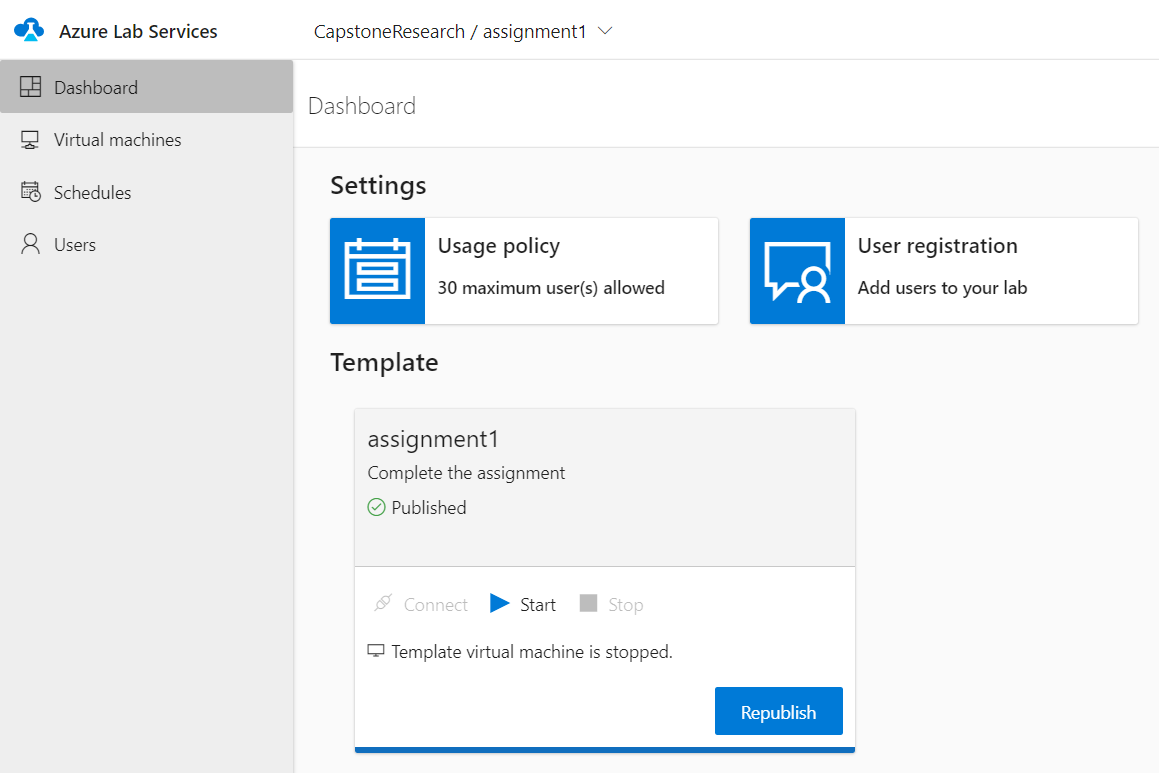
\includegraphics[width=66mm]{img/1.png}
\end{center}
}

\headerbox{Motivation}{name=model,column=0,below=introduction,span=2}{
	We workout often ourselves, and were unsatisfied with the avalible options
	for fitness tracking. In addition we wanted to create an for users who
	are concerned about data privacy, and open source software. We aim to
	provide a drop-in replacement that has all the features and functionality
	of major closed-source competetors.
}

\headerbox{Proposed Solution}{name=mcs,column=0,below=model,span=2}{
Strengthy solves the problem of data at the gym. As a smart and easy way to record data, you can take bigger, better steps to achieving your fitness goals. As time progresses, users will be able to get a clear visualization of the data they've been entering showing their statistics at the gym. With these insights, users can target weak points, and go after goals in areas they want to see improvement in. Many of those involved in regular fitness also typically stick to a routine at the gym, or what some might call a split. These splits we call workouts in our app to allow a user to create an easy to understand format of their routine while at the gym. We also wanted to accomodate for users who do timer-based workouts. For instance, some common exercises that use a timer are the 'plank' and the 'sprint'. Strengthy allows you to set a time for your activity and start a timer based for that activity. Since you may one do more than one sprint or plank, you can add sets accordingly while working out. The same goes with rep-based workouts too, to provide the ease of getting more work in on days you feel more ready to go at the gym. Users can now view their data without the cost of their privacy, their personal information, or their money. Since our solution is open source, users can self-host the platform on their own machine with just a few commands in the command prompt.
}

\headerbox{Results}{name=screen,column=2,span=1,below=info}{ % To reduce this block to 1 column width, remove 'span=2'

\begin{center}
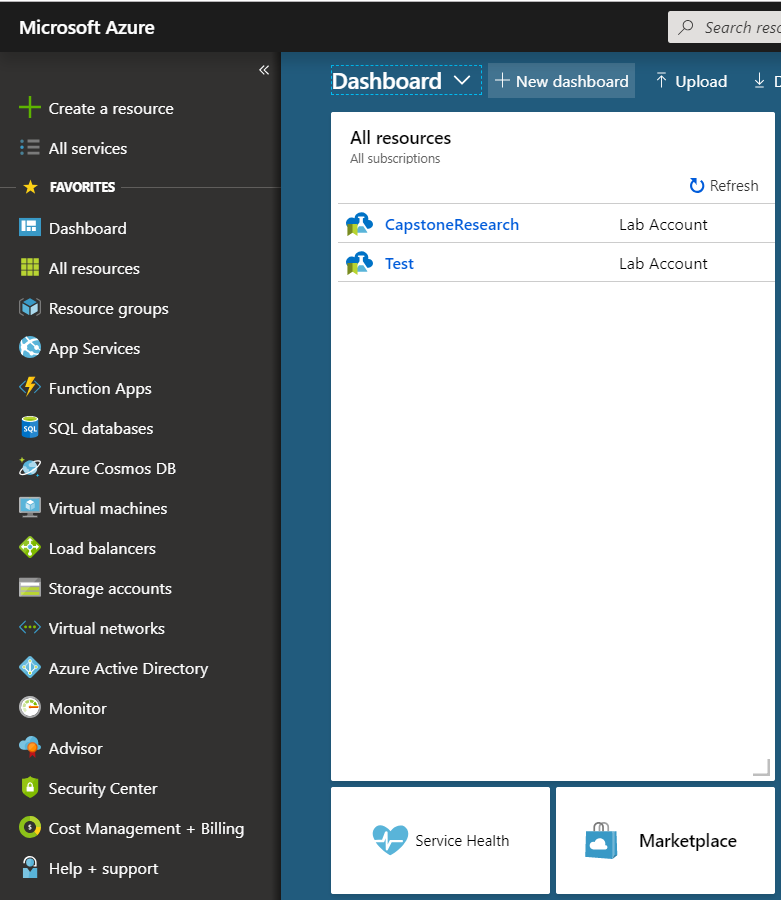
\includegraphics[width=60mm]{img/2.png}
\end{center}

}

\headerbox{Conclusions and Future Work}{name=sea,span=3,column=0,below=mcs}{
%\includegraphics[width=151mm]{GUI1_revised.jpg}
From the beginning, we were looking for a good solution to know what our data looked like at the gym. For awhile it was neglected, but as time went on, seeing graphs and figures showed to be in direct correlation to our success at the gym. While we were able to include basic functionality, it would be interesting to see what we can do with the data once we have it and expand upon it further.
}

\end{poster}

\end{document}
